\documentclass[12 pt]{article}

\usepackage{stoversymb}
\usepackage[margin=0.75in, top=0.875in, bottom=0.875in]{geometry}
\usepackage{amsmath,amsfonts,amssymb,url,multicol,graphicx,tikz,soul}
%===makes urls render well===
\usepackage{lmodern}
\usepackage[T1]{fontenc}
%============================
\usepackage{wasysym} % smileys
\usepackage[inline]{enumitem}

\everymath{\displaystyle}

%\setenumerate{itemsep=0.25in}
\setlist[enumerate,1]{label=\arabic*., itemsep=0.375in}
\setlist[enumerate,2]{label={(\alph*)}, itemsep=0.3125in}
\setlist[enumerate,3]{label={\roman*.}}
\setlist[itemize,1]{label=$\circ$, itemsep=0.25in}

\newcommand{\truefalse}[1]{#1\hfill\rule[-1mm]{220pt}{0.75pt}}
\newcommand{\hint}[1]{(\textbf{Hint}: #1)}
\newcommand{\note}[1]{\textbf{Note}: #1}
\newcommand{\infsum}[3]{\sum_{{#1}={#2}}^\infty {#3}}
\newcommand{\axes}[1]{\begin{center}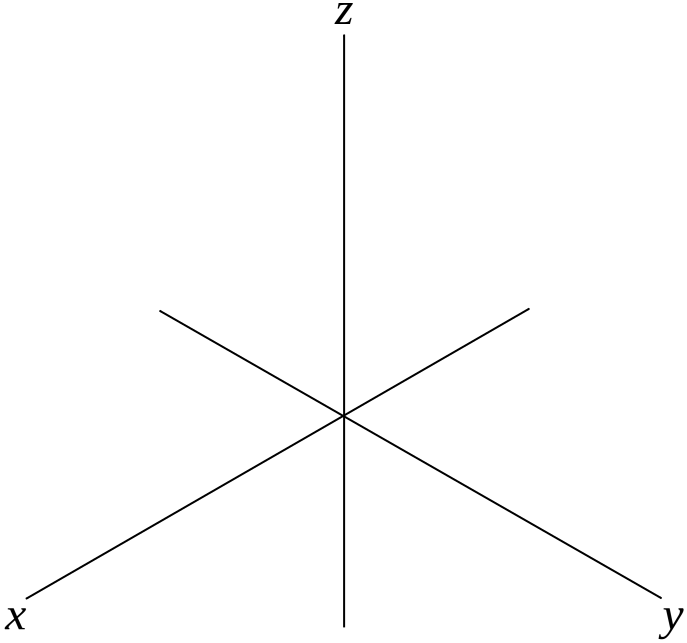
\includegraphics[scale=#1]{3DAxes}\end{center}}
\newcommand{\comps}[1]{\langle #1_1,#1_2,#1_3\rangle}
\newcommand{\compslong}[3]{\langle #1, #2, #3\rangle}
\newcommand{\ijk}[2]{#1\vect{#2}}

\graphicspath{ {./../img/} }
\DeclareGraphicsExtensions{.pdf}

\begin{document}
\begin{flushright}Name: \line(1,0){200}\end{flushright}
\begin{center}
\Large{\textbf{MAC 2313 --- Homework 2}}
\end{center}
\textbf{Directions:} Complete the following problems for a homework grade. Solutions \textit{must} be presented in a neat and professional manner in order to receive credit, answers given without showing work will not be eligible to receive partial credit, and \textit{work for the problems \textbf{must} be done on scratch paper and not on this handout!} \textbf{Date Due:} Tuesday, February 28 (\textit{Use this to study!!})
\vspace{0.25in}
\begin{enumerate}[leftmargin=0in, rightmargin=-0.25in]
%	%========Slack==============
%	\item This question is going to test your ability to do the math we've done in class on a function of your choosing. \textit{This question \ul{will} be graded!}
%	\begin{enumerate}
%			\item Pick your favorite two variable function $f(x,y)$ which is \textit{undefined at (at least) one point}. Call this point $(a,b)$. \note{Don't pick the same function as anyone else!} \vspace{-0.25in}
%			\item Write your function here. \note{You \ul{can't} use a function we examined in class, but you can use those as templates to create your own!}
%			\vspace{0.375in}
%			\item Go to the \texttt{\#your\_functions} channel in our course's \textsc{Slack} room (see course homepage for the URL) and discuss the following:
%			\begin{itemize}		
%				\item Does $\textstyle\lim_{(x,y)\to(a,b)}f(x,y)$ appear to exist? Why or why not? \vspace{3mm}
%				
%				\note{You can use any visualization tool (Wolfram|Alpha \& other 3D graphing tools and/or computer algebra systems) to help your intuition}. Can you prove your claim?
%				\item What are $f_x$ and $f_y$? Does $f_x(a,b)$ or $f_y(a,b)$ exist?
%				\item What are the critical points for your $f$? Does it have any local maxima or minima?
%			\end{itemize}
%	\end{enumerate}
%	\vspace{-0.125in}
	
	\item Let $f(x,y)=3x^2+2xy-y^3$, let $g(x,y)=-x^3+x+y+2y^2$, let $\vect{v}=\langle 3,4 \rangle$, and let $\vect{u}$ be the unit vector in the direction of $\vect{v}$. \note{On your exam, you \textit{will} have to do questions like (b) and (d), and I \textit{won't} give you the formulas!}
	\begin{enumerate}[itemsep=0.625in]
		\item Using any technique you know (e.g. witchcraft, voodoo magic, derivative rules,...), find $f_x$ and $f_y$.
		\item Use the limit definitions
		$$f_x(x,y)=\lim_{h\to0}\frac{f(x+h,y)-f(x,y)}{h} \quad\quad\quad f_y(x,y)=\lim_{h\to0}\frac{f(x,y+y)-f(x,y)}{h}$$
		to find $f_x$ and $f_y$. Does this match your answer for (a)?
		\item Using any technique you know (e.g. witchcraft, voodoo magic, gradient thangs,...), find $D_{\vect{u}}f(x,y)$.
		\item Use the limit definition
		$$D_{\vect{u}}f(x,y)=\lim_{h\to0}\frac{f(x+ah,y+bh)-f(x,y)}{h}$$
		to find $D_{\vect{u}}f(x,y)$. Does this match your answer for (c)?
		\item Are $f$ and/or $g$ differentiable? Why or why not?
	\end{enumerate}

	\newpage
	
%	\item Find each of the indicated partials for $f(x,y,z)=x^2+y^2+z^2+xy + yz + xz - 3xyz+z\sin{x}$.
%	\begin{enumerate}[itemsep=0.725in]
%		\item $f_x$
%		\item $f_{xz}$
%		\item $f_{xzy}$
%		\item $f_y$
%		\item $f_{yy}$
%		\item $f_{yzx}$
%		\item $f_z$
%		\item $f_{zx}$
%		\item $f_{zxy}$
%	\end{enumerate}

	\item Let $f(w,x,y,z)=x^2+y^2+z^2+xy + yz + xz - 3xyz$, where $w=2r^2+s$, $x=2s^2+r-t$, $y=r^2s+t$, and $z=se^r-2\sqrt{t}$. Find each of the following. \note{$w$ also has $t$'s in it, it just has $0$ of them....}
	\begin{enumerate}[itemsep=0.675in]
		\item $\frac{\partial f}{\partial w}$
		\item $\frac{\partial f}{\partial x}$
		\item $\frac{\partial f}{\partial y}$
		\item $\frac{\partial f}{\partial z}$
		\item $\frac{\partial f}{\partial r}$
		\item $\frac{\partial f}{\partial s}$
		\item $\frac{\partial f}{\partial t}$
		\item $\frac{\partial^2 f}{\partial r\,\partial t}$
	\end{enumerate}

	\newpage
	
	\item Let $f(x,y)=\cos(x y)$.
	\begin{enumerate}[itemsep=0.55in]
		\item Find $\nabla f(x,y)$.
		\item Find the equation of the tangent plane to $z=f(x,y)$ at the point $\left(\frac{\pi}{2},\frac{1}{2},\frac{1}{\sqrt{2}}\right)$.
		\item How many critical points does $f$ have, and how do you know?
		\item Is $(0,0,1)$ a critical point of $f$? How do you know?
		\item Could the point $(2,3,f(2,3))$ be a critical point of $f$? Why or why not?
		\item Find $f_{xx}$, $f_{xy}$, $f_{yx}$, and $f_{yy}$.
		\item Use (g) to find $D(x,y)=\det\left(\begin{array}{cc}f_{xx} & f_{xy} \\[3mm] f_{yx} & f_{yy}\end{array}\right)$.
		\item $(0,1,1)$ \textit{is} a critical point of $f$. Is it a local max, local min, or saddle point? How do you know?
		\item Let $\Sigma=\{(x,y)\text{ in }\Reals^2\text{ such that }-1\leq x\leq 1\text{ and }-1\leq y\leq 1\}.$
		Does $f$ attain an absolute maximum on $\Sigma$? An absolute minimum? How do you know?
		\item Find the absolute maximum and absolute minimum of the function $f$ on the closed triangular region $\Delta$ with vertices $(2,0)$, $(0,2)$, and $(0,-2)$.
	\end{enumerate}
%
%	\newpage
%	
%	\item Find the extreme values of $f$ subject to the given constraint or constraints.
%	\begin{enumerate}[itemsep=1in]
%		\item $f(x,y)=x^2+y^2$; $xy=1$
%		\item $f(x,y,z)=yz+xy$; $xy=1$, $y^2+z^2=1$\vspace{0.5in}
%	\end{enumerate}
%
%	\item The plane $x+y+2z=2$ intersects the paraboloid $z=x^2+y^2$ in an ellipse. Find points on this ellipse that are nearest to and farthest from the origin.

	

%	\item Write the vector from $(0,1,2)$ to $(1,\pi,-4)$ in terms of the standard basis vectors $\vect{i}$, $\vect{j}$, and $\vect{k}$.
%	
%	\item Consider the vectors $\vect{u}=\langle -2,3,1\rangle$, $\vect{v}=\vect{i}+\vect{j}+\vect{k}$, and $\vect{w}=\langle 0,-1,-1 \rangle$. Determine whether each of the following quantities is a scalar or a vector, and express each vector with respect to $\vect{i}$, $\vect{j}$, and $\vect{k}$.
%	%\begin{multicols}{2}
%	\begin{enumerate}
%		\item $\vect{v}+\vect{w}$
%		\item $3\vect{v}$
%		\item $\left(\vect{u}\cdot\vect{w}\right)\vect{v}$
%		\item The unit vector in the same direction as $\vect{u}+\vect{w}$
%		\item $\left(\vect{w}\cdot\vect{w}\right)\vect{w}$
%		\item $\vect{w}\times\vect{u}$
%		\item $\vect{u}\times\vect{w}$
%		\item The angle between $\vect{u}+\vect{w}$ and $\vect{u}\times\vect{w}$.
%		\item The unit vector in the same direction as $\vect{w}\times\vect{u}-\vect{u}\times\vect{w}$
%		\item $|\vect{v}-\vect{w}|$
%		\item $|\vect{v}\times\vect{u}|$
%		\item The unit vector orthogonal to both $\vect{u}+3\vect{v}$ and $2\vect{w}$
%		\item The area of the parallelogram spanned by $\vect{u}+\vect{i}$ and $-2\vect{w}$
%		\item $\comp_{\vect{u}}\vect{v}$ and $\proj_{\vect{u}}\vect{v}$ 
%	\end{enumerate}
%
%%	\item Describe the regions in $\Reals^3$ represented by each of the following. Give as much detail as possible (e.g. what're the center/radius of the sphere? what coordinate plane is the plane parallel to? etc.)
%%	\begin{enumerate}
%%		\item $3x^2+3y^2+3z^2=10+6y+12z$
%%		\item $z=x$
%%		
%%	\end{enumerate}
%	\item Let $\vect{a}=\langle a_1,a_2,a_3\rangle$, $\vect{b}=\langle b_1,b_2,b_3\rangle$, $\vect{c}=\langle c_1,c_2,c_3\rangle$, $\vect{u}=\langle u_1,u_2,u_3\rangle$, and $\vect{v}=\langle v_1,v_2,v_3\rangle$ be arbitrary vectors in $\Reals^3$. Prove each of the following.
%	\begin{enumerate}[itemsep=0.95in]
%		\item $\vect{i}\cdot\vect{j}=\vect{j}\cdot\vect{k}=\vect{k}\cdot\vect{i}=0$
%		\item $\vect{i}\cdot\vect{i}=\vect{j}\cdot\vect{j}=\vect{k}\cdot\vect{k}=1$
%		\item The vector $\vect{b}-\proj_{\vect{a}}\vect{b}$ is orthogonal to $\vect{a}$
%		\item $|\vect{a}+\vect{b}|^2+|\vect{a}-\vect{b}|^2=2|\vect{a}|^2+2|\vect{b}|^2$
%		\item $\vect{a}\times(\vect{b}\times\vect{c})=(\vect{a}\cdot\vect{c})\vect{b}-(\vect{a}\cdot\vect{b})\vect{c}$
%		\item $(\vect{u}\times\vect{v})\cdot(\vect{a}\times\vect{b})=(\vect{u}\cdot\vect{a})(\vect{v}\cdot\vect{b})-(\vect{v}\cdot\vect{a})(\vect{u}\cdot\vect{b})$
%		\item $(\vect{u}\times\vect{v})\times\vect{w}+(\vect{v}\times\vect{w})\times\vect{u}+(\vect{w}\times\vect{u})\times\vect{v}=\vect{0}$
%	\end{enumerate}
%	
%	\newpage
%	
%	\item Find each of the following.
%	\begin{enumerate}
%		\item The equation of the line passing through $(2,1,-3)$ and $(6,-1,-5)$.
%		\item The equation of the line passing through $(3,-1,2)$ in the direction of $\ijk{2}{i}-\ijk{3}{j}+\ijk{4}{k}$.
%		\item The equation of the line through $(1,-1,4)$ and perpendicular to both $\vect{i}+\vect{j}-\vect{k}$ and $\compslong{0}{-3}{4}$.
%		\item The equation of the plane passing through $(1,1,1)$ with normal vector $\vect{n}=\ijk{2}{i}+\ijk{}{j}-\ijk{2}{k}$.
%		\item A unit normal vector to the plane $3x+y-z=10$.
%		\item The equation of the plane through the point $(3,-1,-1)$ and perpendicular to the vector $\ijk{}{i}-\ijk{2}{j}+\ijk{}{k}$.
%		\item The equation of the line through $(1,1,1)$ and orthogonal to the plane containing $(0,1,0)$, $(1,0,0)$, and $(0,0,1)$.
%		\item The angle between the planes $x+y+z=1$ and $-x-6y+z=4$.
%		\item The (curve formed by the) intersection of the two-sheet hyperboloid $-x^2+\frac{1}{4}y^2-\frac{1}{2}z^2=1$ and the plane $z=x-\frac{1}{10}y$ (see figures below).  \textbf{Simplify fully!}
%	\end{enumerate}
%	\vfill
%	\begin{center}
%		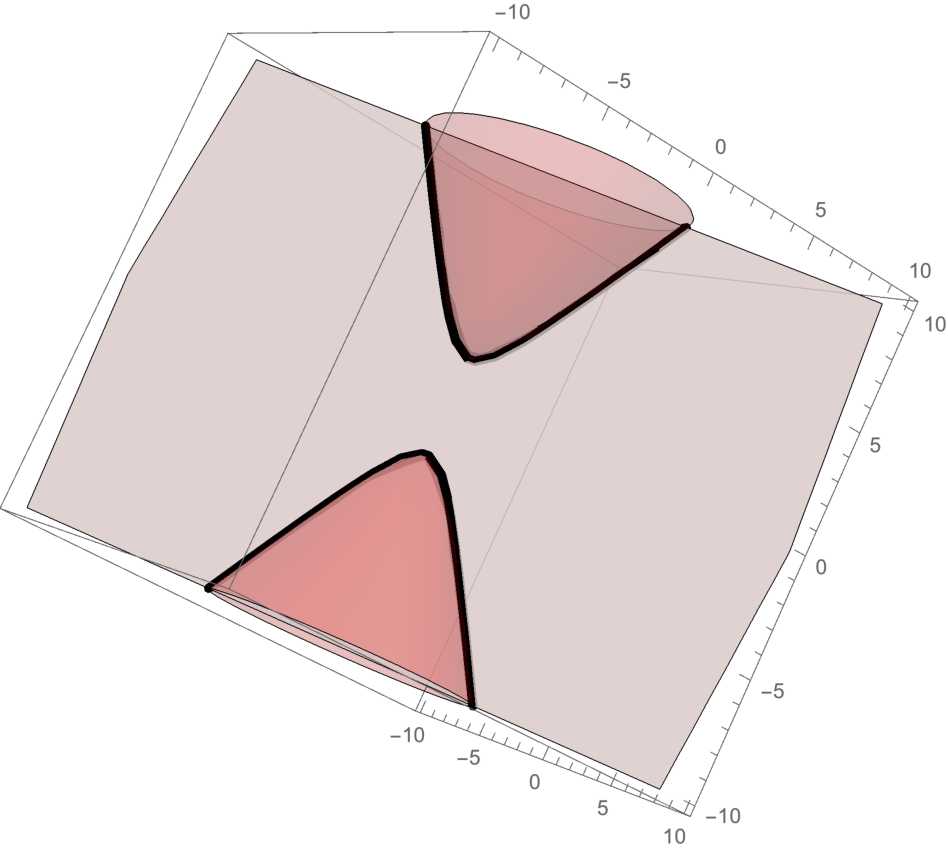
\includegraphics[scale=0.44]{PlaneHyperboloid}\hspace{1in}
%		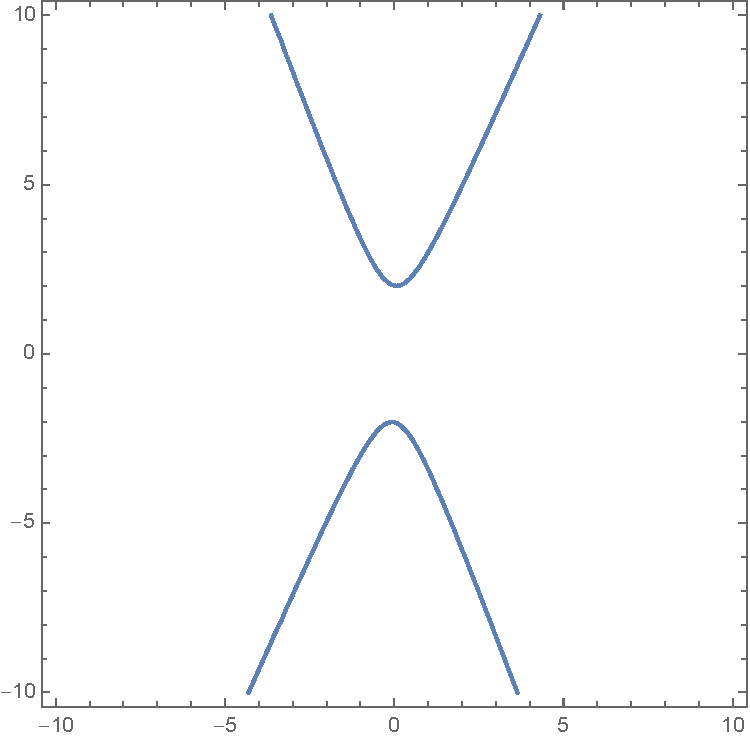
\includegraphics[scale=0.45]{PlaneHyperboloid2}
%	\end{center}
\end{enumerate}
\end{document}